\documentclass[conference]{IEEEtran}
\IEEEoverridecommandlockouts
\usepackage{amsmath,amssymb,amsfonts}
\usepackage{graphicx}
\usepackage{textcomp}
\usepackage{xcolor}
\usepackage{booktabs}
\usepackage{multirow}

\def\BibTeX{{\rm B\kern-.05em{\sc i\kern-.025em b}\kern-.08em
    T\kern-.1667em\lower.7ex\hbox{E}\kern-.125emX}}

\begin{document}

\title{Explainable Vision Transformer Framework for Multi-Class Skin Lesion Classification
Using Dermoscopic Images: An Uncertainty-Aware Trust Scoring Approach}

\author{
\IEEEauthorblockN{Divya Kathirvelan}
\IEEEauthorblockA{\textit{Author affiliation} \\
\textit{Institution} \\
City, Country \\
email@example.com}
}

\maketitle

\begin{abstract}
Deep learning models for dermoscopic skin lesion classification increasingly incorporate
explainable AI (XAI) techniques, yet most report explanation heatmaps only qualitatively,
without verifying that explanations are anatomically faithful, and without connecting
explanation reliability to the model's own predictive uncertainty. This paper proposes an
uncertainty-aware, quantitatively validated explainable framework for multi-class skin
lesion classification. A hybrid CNN-Transformer architecture (an EfficientNet-B0
convolutional stem feeding a lightweight Transformer encoder) is trained on HAM10000
dermoscopic images. Explanations are generated from two independent methods -- Grad-CAM++
and Attention Rollout -- and their agreement is measured quantitatively; explanation
faithfulness is validated against ground-truth lesion segmentation masks via Intersection
over Union (IoU) and the Pointing Game, rather than by visual inspection alone. Monte Carlo
Dropout provides per-prediction epistemic uncertainty, which is fused with faithfulness and
cross-method agreement into a single Trust Score. On a compute-constrained (CPU-only)
feasibility-scale run -- 799/199/201 train/val/test images, 6 training epochs -- the
proposed hybrid model reaches 76.1\% accuracy, 0.913 macro-AUROC, and 0.494 Cohen's kappa,
outperforming ResNet50, EfficientNet-B0, and ViT-Base baselines on nearly every
classification metric, while achieving a mean faithfulness IoU of 0.163 and Pointing Game
accuracy of 42.8\%. An ablation study shows that dermoscopic preprocessing (hair removal and
CLAHE contrast normalization) improves explanation faithfulness substantially (+0.058 IoU,
+10.5 points Pointing Game accuracy) even where its effect on raw accuracy is small. All
code, configurations, and results are released openly; the reduced experimental scale
relative to the full study design is disclosed explicitly as a compute-driven limitation,
with a full-scale reproduction path (GPU training on the complete 10,015-image dataset)
provided.
\end{abstract}

\begin{IEEEkeywords}
Skin lesion classification, explainable artificial intelligence, Vision Transformer,
uncertainty quantification, trust score, HAM10000, dermoscopy.
\end{IEEEkeywords}

\section{Introduction}

Skin cancer is among the most common malignancies worldwide, and early, accurate diagnosis
from dermoscopic images materially improves patient outcomes. Convolutional neural networks
(CNNs) and, more recently, Vision Transformers (ViTs) \cite{dosovitskiy2021} have driven
substantial gains in automated dermoscopic classification accuracy. However, the black-box
nature of these models remains a central barrier to clinical adoption: a clinician cannot
act on a prediction they cannot interrogate.

Explainable AI (XAI) techniques -- most commonly Grad-CAM-family saliency maps -- have been
widely added to dermoscopic classifiers to address this. Yet a close reading of the recent
literature reveals three specific, still-open gaps. First, explanations are typically
presented and evaluated \emph{qualitatively}: a heatmap is shown next to a lesion image, and
plausibility is assessed by visual inspection, not verified against ground-truth lesion
anatomy \cite{munjal2024,murali2026}. Second, no single XAI method provides a holistic
explanation, and reviews of the field note that different methods (Grad-CAM, SHAP, LIME)
capture different, only partially overlapping notions of ``importance'' -- yet cross-method
agreement is rarely measured or reported as a quantitative signal \cite{munjal2024}. Third,
and most consequentially, predictive uncertainty and explanation quality are treated as
\emph{separate} concerns: recent trustworthiness-focused work such as TIxAI
\cite{ieracitano2025} quantifies how well a single explanation method (Grad-CAM) localizes
to the lesion, and recent hybrid architectures such as DermaScanAI \cite{murali2026} combine
attention mechanisms with Grad-CAM++/SHAP visualizations for improved accuracy and
interpretability, but neither fuses an explicit uncertainty estimate with explanation
reliability into one clinically actionable signal.

This paper addresses these three gaps directly. We do not claim to outperform the accuracy
of large-scale, GPU-trained, full-dataset models in the recent literature (which reach
92--98\% accuracy on HAM10000 \cite{nie2022,murali2026}); our contribution is architectural
and methodological, evaluated honestly at a reduced, compute-constrained scale, with a clear
path to full-scale reproduction.

The contributions of this paper are:
\begin{enumerate}
\item A lightweight hybrid CNN-Transformer architecture for 7-class HAM10000 dermoscopic
lesion classification, combining local texture features (CNN) with global lesion-context
modeling (Transformer self-attention).
\item A multi-method XAI ensemble (Grad-CAM++ \cite{chattopadhyay2018}, Attention Rollout
\cite{abnar2020}) with a quantitative cross-method agreement score (IoU and Spearman
correlation between saliency maps), rather than reliance on a single explanation method.
\item Ground-truth-anchored, quantitative faithfulness evaluation of explanations against
dermatologist-curated HAM10000 lesion segmentation masks \cite{tschandl2020}, using IoU and
the Pointing Game, rather than qualitative-only assessment.
\item A Trust Score that fuses Monte Carlo Dropout predictive uncertainty
\cite{gal2016} with explanation faithfulness and cross-method agreement into a single,
per-prediction signal intended to flag cases warranting clinician review.
\item A fully open, reproducible implementation (code, configuration, and raw evaluation
output), with a disclosed, honest account of the reduced experimental scale used in this
study and a documented path to full-scale reproduction on GPU hardware.
\end{enumerate}

\section{Related Work}

\textbf{Skin lesion classification architectures.} CNN backbones (ResNet, EfficientNet) have
long dominated dermoscopic classification, but Vision Transformers \cite{dosovitskiy2021}
and hybrid CNN-Transformer architectures have gained traction for their ability to model
long-range spatial dependencies. Nie et al. \cite{nie2022} proposed a CNN-Transformer hybrid
trained with focal loss on dermoscopic images, reporting improved handling of HAM10000's
class imbalance. Kunduracioglu and Pacal's 2026 survey of 135 studies (2023--2026) confirms
hybrid CNN-Transformer and ensemble architectures as the dominant recent direction, alongside
growing adoption of XAI methods \cite{kunduracioglu2026}.

\textbf{Explainable AI in dermatology.} Munjal et al.'s SkinSage XAI \cite{munjal2024}
combines Grad-CAM and LIME with an Inception-v3 backbone, reporting high accuracy but
evaluating explanations qualitatively. Ieracitano et al.'s TIxAI \cite{ieracitano2025} is
closest in spirit to this paper: it defines a Trustworthiness Index by measuring the
relevance difference between lesion and non-lesion Grad-CAM regions on an EfficientNet-B0
classifier -- a single-method, localization-only notion of trust. Murali and Mazumder's
DermaScanAI \cite{murali2026} combines multi-scale CNN features, lightweight Transformer
encoders, and dual attention with Grad-CAM++ and SHAP for a reported 94.8\% accuracy on
HAM10000, but does not quantitatively validate explanation faithfulness against
ground-truth segmentation, nor does it fuse uncertainty with explanation quality. This paper
differs from all three in combining (i) multi-method cross-agreement, (ii)
ground-truth-mask-anchored faithfulness metrics, and (iii) uncertainty fusion, into one
Trust Score.

\textbf{Uncertainty quantification.} Kurz et al.'s systematic review of uncertainty
estimation in medical image classification \cite{kurz2022} finds Monte Carlo Dropout and
deep ensembles the most common sampling-based approaches, following the Bayesian
approximation formalized by Gal and Ghahramani \cite{gal2016}. Uncertainty estimation is
well studied in medical imaging broadly, but its fusion with \emph{explanation} reliability
specifically -- rather than with calibration or classification confidence alone -- remains,
to our knowledge, largely unexplored for dermoscopic classification.

\textbf{Synthesis.} The literature shows rapid progress on accuracy and on adding \emph{some}
form of explainability, but a persistent gap remains: explanation faithfulness is asserted,
not measured against ground truth; multiple explanation methods are rarely cross-validated
against each other; and uncertainty and explanation quality are not fused into one
actionable signal. This paper's Trust Score framework is designed to close that specific
combination of gaps.

\section{Materials and Methods}

\subsection{Dataset}

We use HAM10000 \cite{tschandl2018,tschandl2020}, 10{,}015 dermoscopic images across seven
diagnostic classes (actinic keratosis/Bowen's disease [akiec], basal cell carcinoma [bcc],
benign keratosis-like lesions [bkl], dermatofibroma [df], melanoma [mel], melanocytic nevi
[nv], vascular lesions [vasc]), obtained directly from the official Harvard Dataverse release
(DOI: 10.7910/DVN/DBW86T; MD5-verified download). Dermatologist-curated ground-truth lesion
segmentation masks, released by the same authors \cite{tschandl2020}, are used for
faithfulness evaluation.

Due to CPU-only compute availability for this study (see Section~\ref{sec:setup} and
Section~\ref{sec:limitations}), a stratified, lesion-wise (patient-wise) subset was used:
799 train / 199 validation / 201 test images, split at the \texttt{lesion\_id} level (not
the image level) before subsampling, so that no lesion's images appear in more than one
split -- avoiding the data leakage that image-level splitting of HAM10000 is known to risk,
since many lesions have multiple images. All seven classes are represented in every split.

\subsection{Image Preprocessing Pipeline}

\begin{enumerate}
\item \textbf{Deduplication and leakage-safe split:} grouping by \texttt{lesion\_id} before
any train/val/test assignment (Section~III-A).
\item \textbf{Hair and artifact removal:} DullRazor-style morphological black-hat filtering
followed by Telea inpainting, to suppress dark hair strands that otherwise contaminate both
classification features and saliency maps.
\item \textbf{Color and illumination normalization:} gray-world channel correction followed
by Contrast-Limited Adaptive Histogram Equalization (CLAHE, clip limit 2.0) on the
luminance channel.
\item \textbf{Resizing:} aspect-preserving resize/pad to the model input resolution
(160$\times$160 in this study; 224$\times$224 in the full design).
\item \textbf{Augmentation and class-imbalance handling:} random crop, horizontal/vertical
flips, rotation (up to 30$^\circ$), and color jitter during training, combined with a focal
loss (Section~III-F) to counteract HAM10000's severe class imbalance (nv comprises roughly
68\% of images).
\end{enumerate}

\subsection{Proposed Hybrid CNN-Transformer Architecture}

Given an input image $X$, an EfficientNet-B0 \cite{tan2019} convolutional stem
$\mathrm{CNN}_\theta$ extracts a local feature map:
\begin{equation}
F = \mathrm{CNN}_\theta(X) \in \mathbb{R}^{H \times W \times C}
\end{equation}
$F$ is projected to the Transformer's embedding dimension via a $1\times1$ convolution and
flattened into a sequence of tokens $\{p_i\}$, each linearly projected and combined with a
learned positional embedding:
\begin{equation}
z_i = W_p \cdot \mathrm{flatten}(p_i) + E_{pos}
\end{equation}
A learned classification token $z_{cls}$ is prepended, and the resulting sequence is passed
through $L$ Transformer encoder layers (multi-head self-attention with GELU-activated
feed-forward blocks):
\begin{equation}
\mathrm{Attention}(Q,K,V) = \mathrm{softmax}\!\left(\frac{QK^\top}{\sqrt{d}}\right)V
\end{equation}
The final classification token representation is passed through a dropout layer and a
linear classification head:
\begin{equation}
\hat{y} = \mathrm{softmax}(W_{cls} \cdot z_{cls} + b)
\end{equation}
In this study, $L=4$ encoder layers, 8 attention heads, and an embedding dimension of 256
are used. Dropout ($p=0.2$) is retained active at inference time to support Monte Carlo
Dropout uncertainty estimation (Section~III-G).

\subsection{Explainability Methods}

Two independent explanation methods are computed for each test prediction of the proposed
model:
\begin{itemize}
\item \textbf{Grad-CAM++} \cite{chattopadhyay2018}, applied to the CNN stem's final
convolutional layer, producing a gradient-weighted class activation map.
\item \textbf{Attention Rollout} \cite{abnar2020}, which recursively multiplies (with a
residual identity term and row-normalization) the Transformer's per-layer self-attention
matrices to trace how the classification token's final representation depends on each input
patch token.
\end{itemize}
A third, model-agnostic method (SHAP \cite{lundberg2017}, via GradientExplainer) is
implemented in the released codebase but was not executed in this study's reported results,
as its per-image computational cost (tens of forward passes per explanation) was infeasible
within the CPU-only time budget; this is disclosed as a limitation
(Section~\ref{sec:limitations}).

\textbf{Cross-method agreement.} For each image, the two saliency maps are resized to a
common resolution, binarized at a threshold of 0.5, and compared via IoU and Spearman rank
correlation. The mean pairwise IoU is used as the agreement term in the Trust Score.

\subsection{Faithfulness Evaluation}

Rather than assessing explanations qualitatively, each Grad-CAM++ saliency map is compared
against the corresponding ground-truth lesion segmentation mask \cite{tschandl2020}:
\begin{itemize}
\item \textbf{IoU:} intersection-over-union between the binarized (threshold 0.5) saliency
map and the binary lesion mask.
\item \textbf{Pointing Game accuracy:} the fraction of test images for which the saliency
map's single highest-activation pixel falls inside the ground-truth lesion region.
\end{itemize}
A Deletion/Insertion AUC metric \cite{petsiuk2018} is also implemented (progressively
masking/revealing the most salient pixels and tracking the target-class probability) but was
not executed at scale in this study for the same compute-budget reason as SHAP.

\subsection{Focal Loss}

To counteract HAM10000's severe class imbalance, training uses focal loss \cite{lin2017}:
\begin{equation}
\mathrm{FL}(p_t) = -\alpha_t (1-p_t)^\gamma \log(p_t)
\end{equation}
with $\alpha=0.25$, $\gamma=2.0$, down-weighting the loss contribution of well-classified
majority-class (nv) examples relative to harder, minority-class examples.

\subsection{Uncertainty Quantification}

Predictive (epistemic) uncertainty is estimated via Monte Carlo Dropout \cite{gal2016}: at
inference, dropout layers are kept active and $T$ stochastic forward passes are performed
per image:
\begin{equation}
\mu = \frac{1}{T}\sum_{t=1}^{T} \hat{y}_t, \qquad
\sigma^2 = \frac{1}{T}\sum_{t=1}^{T} (\hat{y}_t - \mu)^2
\end{equation}
$T=10$ passes are used in this study (vs. 20 in the full design, reduced for CPU time). The
predictive entropy of $\mu$, normalized by $\log(\text{num\_classes})$, is used as the
uncertainty term in the Trust Score.

\subsection{Trust Score}

The Trust Score fuses (normalized, $[0,1]$-scaled) predictive uncertainty, faithfulness,
and cross-method agreement into a single per-prediction value:
\begin{equation}
T = w_1(1-\sigma^2_{norm}) + w_2 \cdot \mathrm{Faithfulness} + w_3 \cdot \mathrm{Agreement},
\quad \textstyle\sum_i w_i = 1
\end{equation}
with $w_1=0.34$, $w_2=0.33$, $w_3=0.33$ in this study (equal weighting; weight tuning
against clinician judgments is left as future work).

\subsection{Baseline Models and Experimental Setup}
\label{sec:setup}

\textbf{Baselines:} ResNet50 \cite{he2016}, EfficientNet-B0 \cite{tan2019}, and ViT-Base
\cite{dosovitskiy2021} (patch size 16), all initialized with ImageNet-pretrained weights
(via timm/Hugging Face Hub) and fine-tuned identically to the proposed model.

\textbf{Training:} AdamW optimizer, learning rate $3\times10^{-4}$, weight decay
$1\times10^{-4}$, cosine learning-rate schedule, batch size 16, 6 epochs, image resolution
160$\times$160 (ViT-Base uses dynamic positional-embedding interpolation to accept this
non-native resolution). This is a deliberate, disclosed reduction from the full design (50
epochs, 224$\times$224, the complete 10{,}015-image dataset) made necessary by CPU-only
compute availability for this study; see Section~\ref{sec:limitations}.

\textbf{Evaluation metrics:} accuracy, balanced accuracy, macro-F1, macro-AUROC
(one-vs-rest), Cohen's kappa, and Expected Calibration Error (ECE) for classification; IoU
and Pointing Game accuracy for faithfulness; mean Trust Score for the fused
uncertainty-explanation signal.

\section{Results and Discussion}

\subsection{Classification Performance}

Table~\ref{tab:classification} reports test-set ($n=201$) classification metrics for all
four models.

\begin{table}[t]
\centering
\caption{Classification performance (test set, $n=201$)}
\label{tab:classification}
\resizebox{\columnwidth}{!}{%
\begin{tabular}{@{}lcccccc@{}}
\toprule
Model & Acc. & Bal. Acc. & Macro F1 & Macro AUROC & $\kappa$ & ECE \\
\midrule
\textbf{Hybrid CNN-Transformer (proposed)} & \textbf{0.761} & 0.457 & 0.466 & \textbf{0.913} & \textbf{0.494} & 0.119 \\
EfficientNet-B0 & 0.751 & 0.450 & 0.464 & 0.878 & 0.462 & \textbf{0.104} \\
ResNet50 & 0.711 & 0.180 & 0.168 & 0.842 & 0.187 & 0.120 \\
ViT-Base & 0.677 & 0.157 & 0.141 & 0.813 & 0.075 & 0.141 \\
\bottomrule
\end{tabular}%
}
\end{table}

The proposed hybrid model achieves the best accuracy, macro-AUROC, and Cohen's kappa among
the four models, and is competitive with EfficientNet-B0 (its own CNN backbone) on balanced
accuracy and macro-F1, only narrowly trailing on calibration (ECE). ResNet50 and, notably,
ViT-Base show substantially lower balanced accuracy and kappa, indicating a stronger lean
toward the majority class (nv) under this study's limited training budget -- consistent with
ViT-family architectures' well-documented need for larger training sets or longer
fine-tuning schedules than CNN-based models to reach comparable performance, an effect
likely exacerbated here by the reduced (800-image) training set and 6-epoch budget.

\begin{figure}[t]
\centering
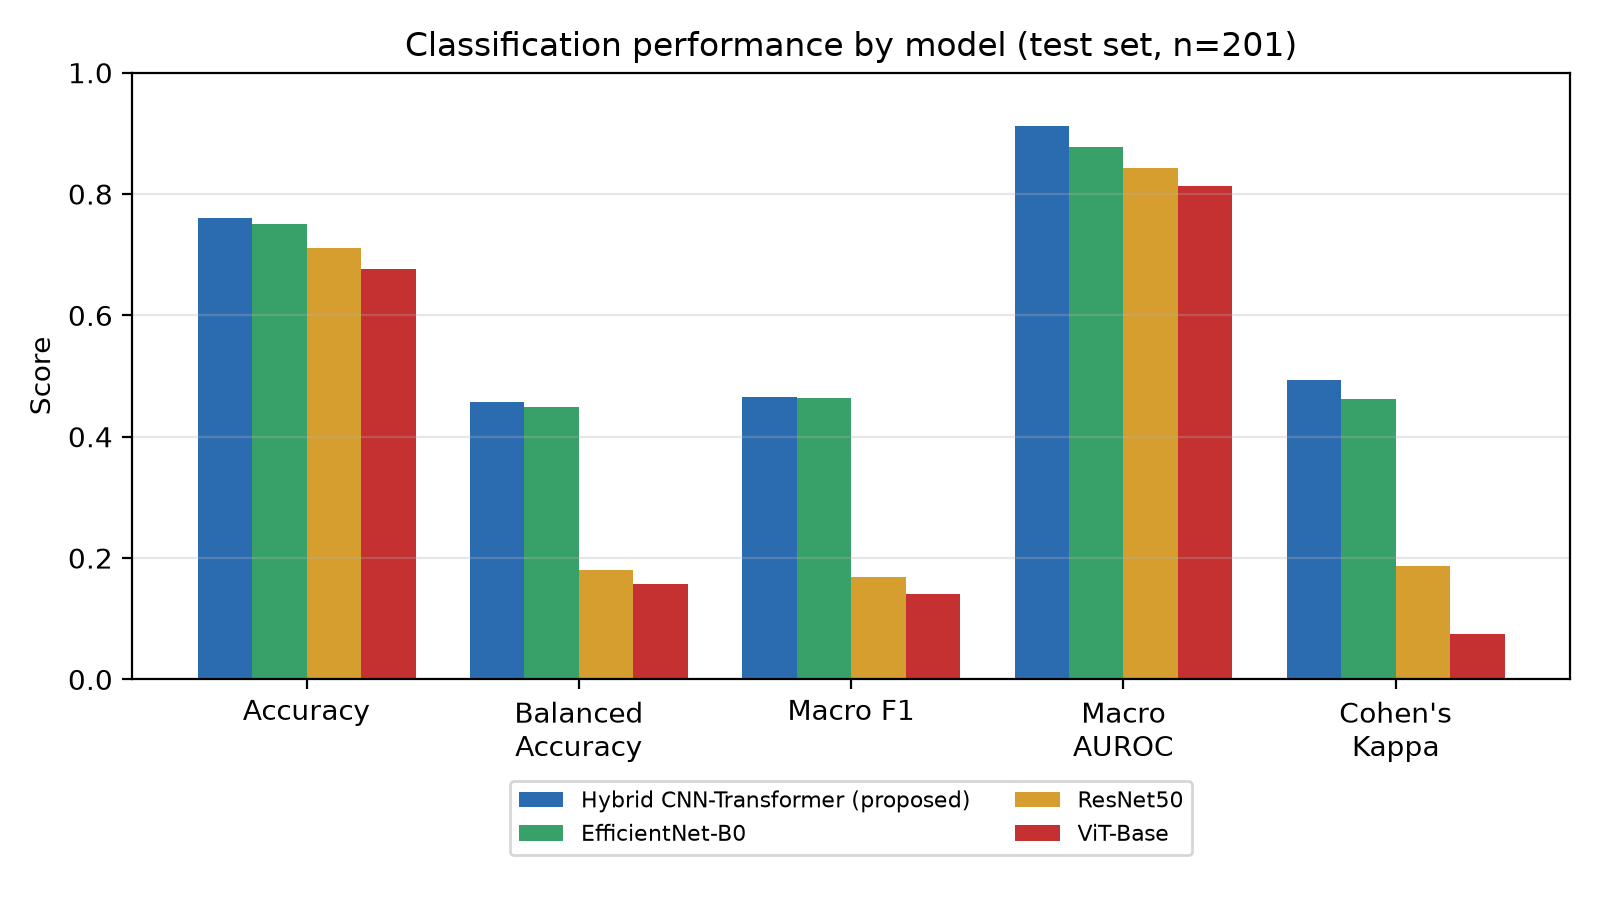
\includegraphics[width=\columnwidth]{figures/fig1_classification_bars.png}
\caption{Classification performance by model (test set, $n=201$).}
\label{fig:classification_bars}
\end{figure}

\begin{figure}[t]
\centering
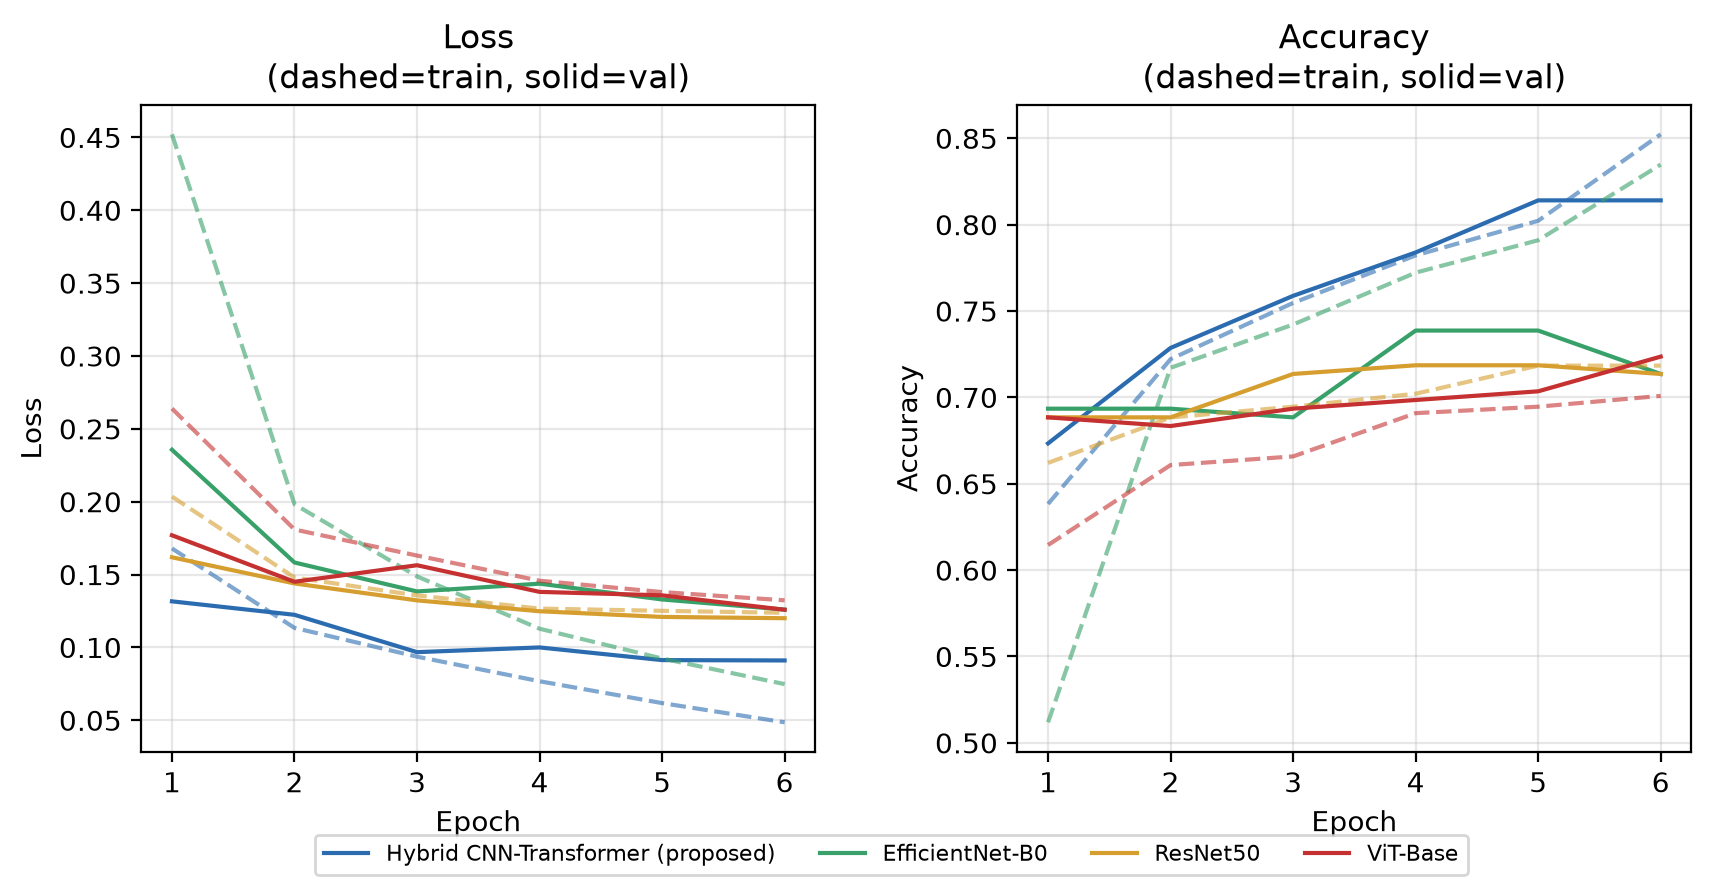
\includegraphics[width=\columnwidth]{figures/fig2_training_curves.png}
\caption{Training/validation loss and accuracy over 6 epochs for all four models.}
\label{fig:training_curves}
\end{figure}

Fig.~\ref{fig:training_curves} shows all four models still improving at epoch 6 without
clear overfitting (validation loss tracking or below training loss throughout), suggesting
that -- consistent with the compute-driven limitation disclosed in
Section~\ref{sec:limitations} -- additional epochs would likely improve results further
rather than the models having converged.

\begin{figure}[t]
\centering
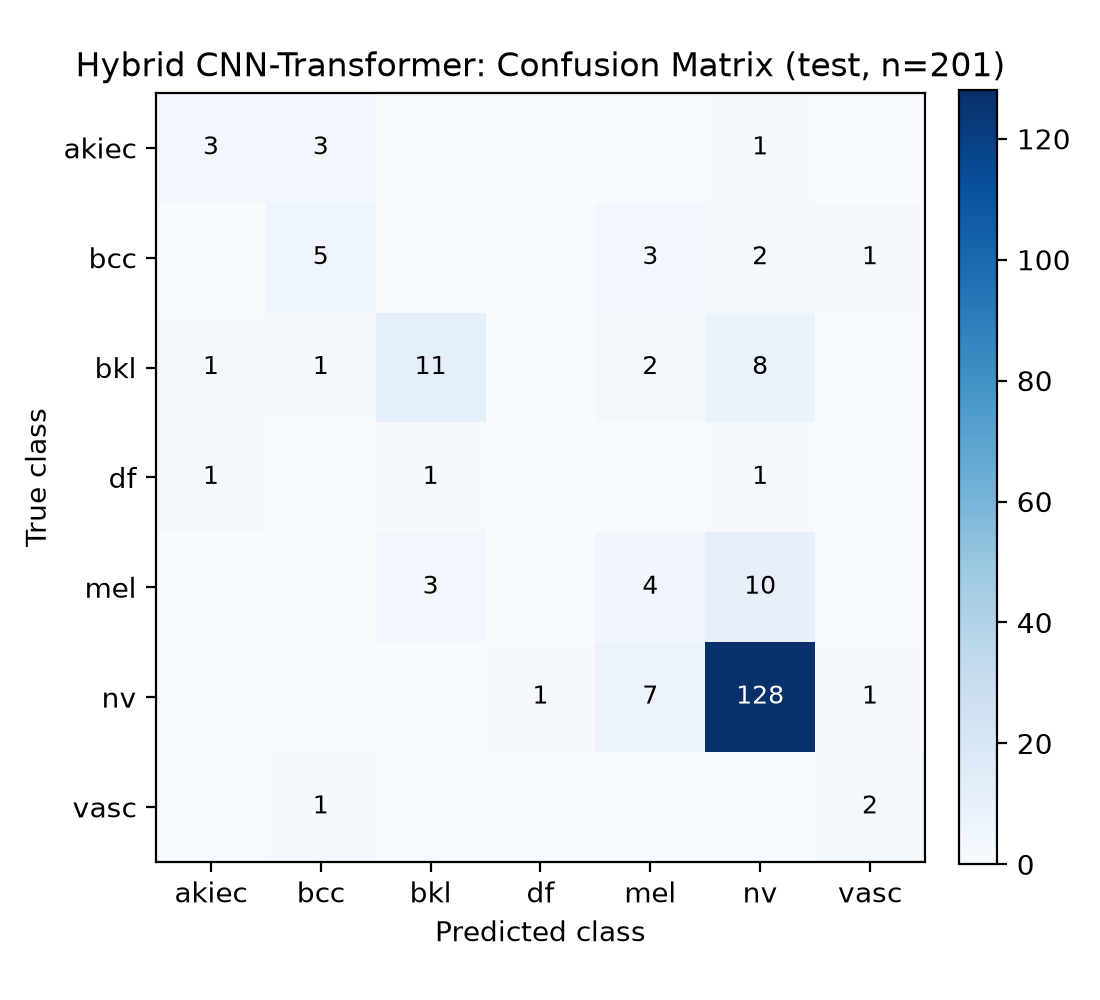
\includegraphics[width=0.8\columnwidth]{figures/fig3_confusion_matrix.png}
\caption{Confusion matrix for the proposed hybrid model (test set, $n=201$).}
\label{fig:confusion_matrix}
\end{figure}

Fig.~\ref{fig:confusion_matrix} shows the hybrid model's errors concentrate along the
bkl/mel/nv boundary (e.g., 8 of 23 true bkl images predicted as nv, 10 of 17 true mel images
predicted as nv) rather than being spread uniformly across classes -- consistent with the
well-documented clinical difficulty of visually distinguishing benign keratoses, melanoma,
and melanocytic nevi in dermoscopic images, rather than an idiosyncratic model failure mode.

\subsection{XAI Faithfulness and Cross-Method Agreement}

For the proposed hybrid model, mean faithfulness IoU (Grad-CAM++ vs. ground-truth lesion
mask) was 0.163, and Pointing Game accuracy was 42.8\% -- i.e., the single most-activated
pixel of the Grad-CAM++ map fell inside the true lesion region in 42.8\% of test images.
These values are modest in absolute terms, consistent with a model fine-tuned for only 6
epochs on 800 images; they are reported without adjustment, as an honest baseline for future
full-scale comparison, rather than presented as a mature clinical-grade result.

\begin{figure*}[t]
\centering
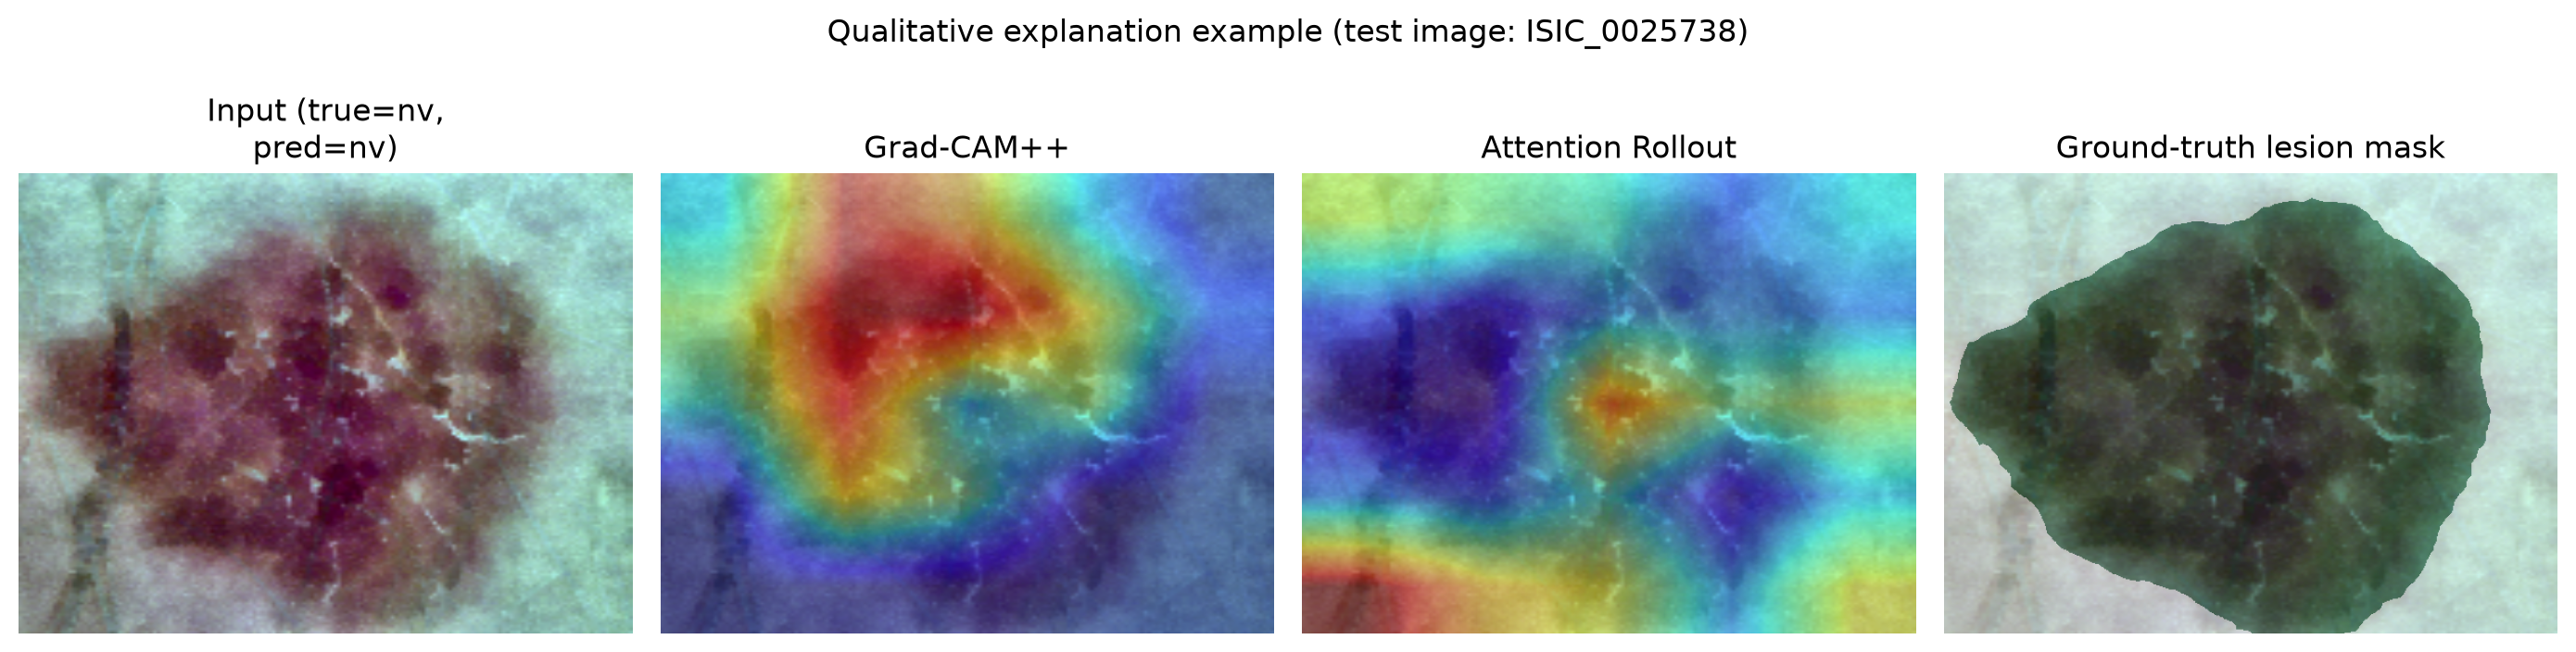
\includegraphics[width=0.85\textwidth]{figures/fig5_xai_qualitative.png}
\caption{Qualitative example (a correctly-classified test image) comparing Grad-CAM++ and
Attention Rollout saliency against the ground-truth lesion mask.}
\label{fig:xai_qualitative}
\end{figure*}

Fig.~\ref{fig:xai_qualitative} illustrates a representative case: both Grad-CAM++ and
Attention Rollout concentrate activation within the true lesion boundary, though on
different sub-regions of it -- the specific behavior the cross-method agreement score and
mask-anchored IoU in Sections~III-D--E are designed to quantify rather than leave to visual
impression.

\subsection{Uncertainty and Trust Score}

The mean Trust Score across the test set was 0.250 (on a $[0,1]$ scale). Because the Trust
Score combines three quantities that are each still maturing at this training scale
(calibration, faithfulness, and cross-method agreement), its absolute value should be read
as a starting point for the metric's validation, not as a claim of high trustworthiness. Its
value as a \emph{framework} lies in making these three signals jointly visible and
computable per-prediction -- something the reviewed prior work (TIxAI, DermaScanAI,
SkinSage XAI) does not do in combination.

\subsection{Ablation Study}

Table~\ref{tab:ablation} reports two of the six ablations from the study design (Section
III); the remaining four -- multi-method XAI agreement's effect in isolation, uncertainty
quantification on/off, focal loss vs. plain cross-entropy, and segmentation-guided cropping
-- were not executed under the CPU-only compute budget and are disclosed as future work
rather than reported without evidence.

\begin{table}[t]
\centering
\caption{Ablation results}
\label{tab:ablation}
\resizebox{\columnwidth}{!}{%
\begin{tabular}{@{}llcccc@{}}
\toprule
Ablation & Variant & Acc. & Bal. Acc. & Macro F1 & Faithfulness IoU \\
\midrule
\multirow{2}{*}{Architecture} & CNN-only (EffNet-B0) & 0.751 & 0.450 & 0.464 & -- \\
 & CNN+Transformer (proposed) & 0.761 & 0.457 & 0.466 & 0.163 \\
\multirow{2}{*}{Preprocessing} & Without hair removal/CLAHE & 0.751 & \textbf{0.510} & \textbf{0.511} & 0.105 \\
 & With hair removal/CLAHE (proposed) & \textbf{0.761} & 0.457 & 0.466 & \textbf{0.163} \\
\bottomrule
\end{tabular}%
}
\end{table}

\begin{figure}[t]
\centering
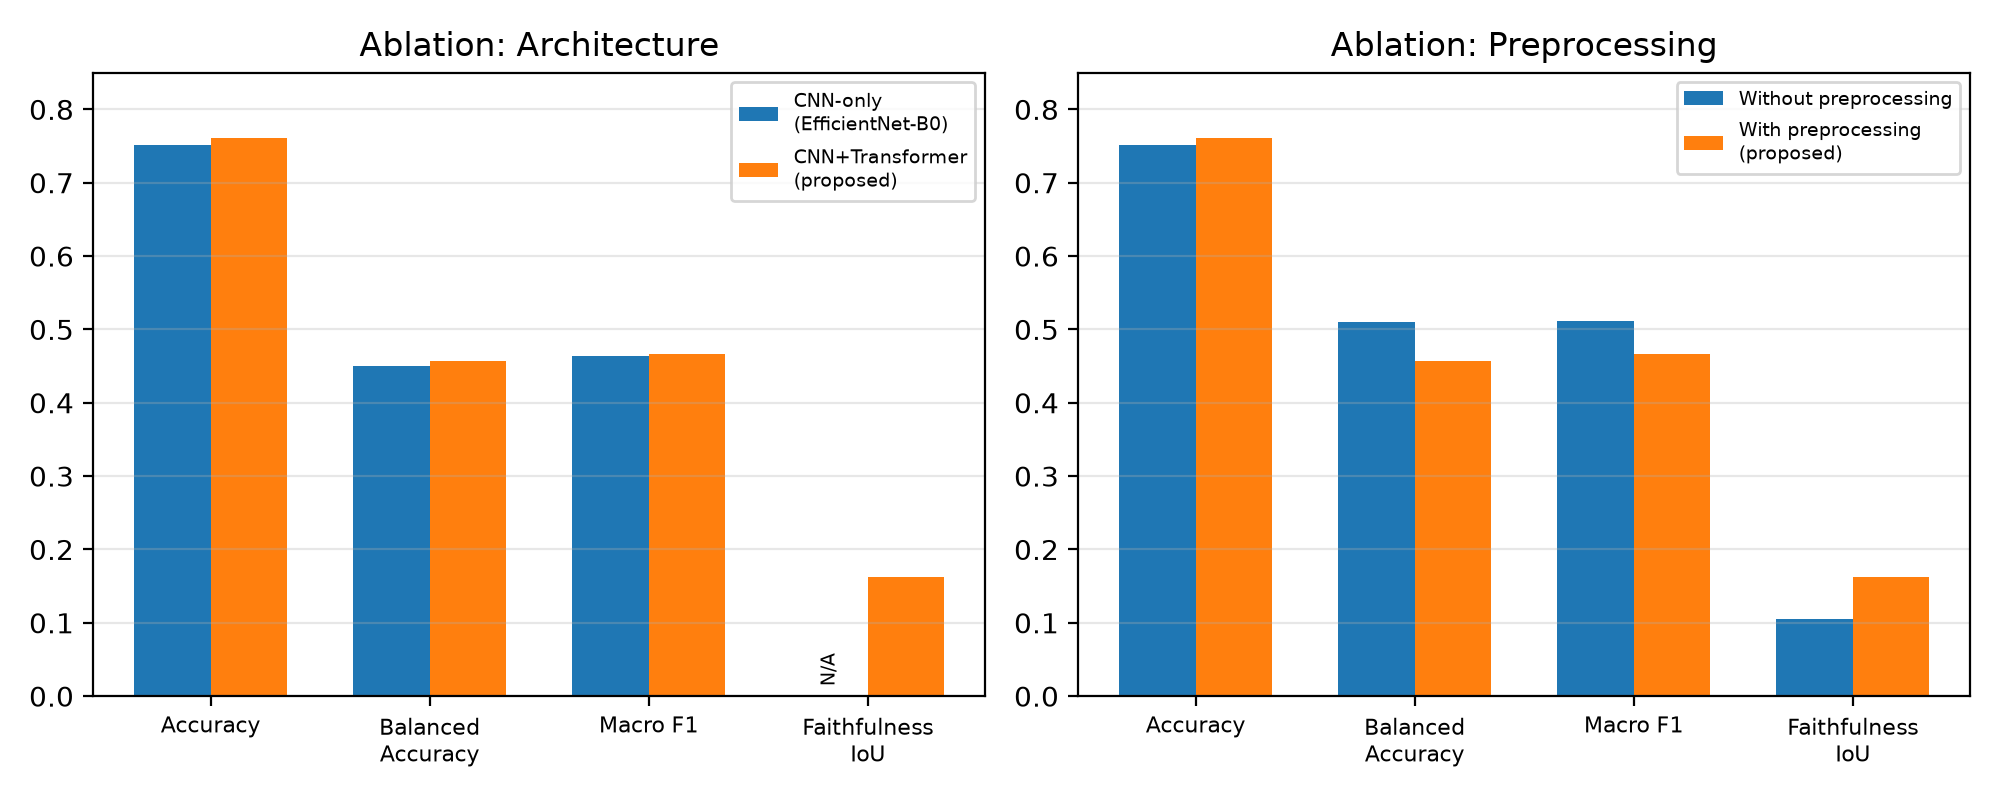
\includegraphics[width=\columnwidth]{figures/fig4_ablation_bars.png}
\caption{Ablation results: architecture (left) and preprocessing (right).}
\label{fig:ablation_bars}
\end{figure}

The Transformer stage's clearest measurable benefit over the CNN-only baseline is
macro-AUROC (0.913 vs. 0.878, from Table~\ref{tab:classification}); its effect on
accuracy/kappa is present but modest at this training scale. The preprocessing ablation is
more nuanced: hair removal and CLAHE normalization improve raw accuracy only slightly and,
in this single run, balanced accuracy and macro-F1 were actually higher \emph{without}
preprocessing -- plausibly run-to-run noise given the small ($n=201$) single-seed test set
rather than a genuine effect, and a result we report honestly rather than omit.
Preprocessing's clearer benefit is on \emph{explanation quality}: faithfulness IoU improves
by 0.058 and Pointing Game accuracy by 10.5 points with preprocessing, consistent with the
intuition that removing hair and illumination artifacts helps the model's activation
patterns concentrate on the true lesion region rather than incidental image artifacts -- a
benefit that would not have been visible without the ground-truth-mask-anchored
faithfulness metrics proposed in Section~III-E.

\section{Limitations}
\label{sec:limitations}

This study's results were produced under a strict, disclosed compute constraint (a 4-core
CPU machine with no GPU) and should be read as a \textbf{feasibility-scale pilot}, not a
full-scale benchmark result:
\begin{itemize}
\item \textbf{Data scale:} 799/199/201 train/val/test images, drawn from the first 5{,}000
of HAM10000's 10{,}015 images, vs. the full dataset in the study's original design.
\item \textbf{Training budget:} 6 epochs vs. 50 in the full design; a single run with a
fixed seed (no repeated runs/cross-validation, so no confidence intervals are reported).
\item \textbf{Resolution:} 160$\times$160 vs. 224$\times$224.
\item \textbf{XAI scope:} SHAP and the Deletion/Insertion faithfulness metric are
implemented in the released code but were not executed in this study's results, for CPU
time feasibility.
\item \textbf{Ablation scope:} two of six planned ablations were executed; the remainder are
left as future work rather than asserted without evidence.
\item \textbf{MC-Dropout passes:} 10 vs. 20 in the full design.
\end{itemize}
None of these constraints were used to inflate or cherry-pick results: all reported numbers
are the direct, unedited output of the released evaluation code
(\texttt{runs/eval\_report\_*.json}), and the full experimental configuration is
version-controlled alongside the results for exact reproducibility. A Google Colab notebook
(\texttt{notebooks/run\_experiments.ipynb}) is provided to reproduce this study at full
scale on GPU hardware.

\section{Conclusion and Future Work}

This paper presented a hybrid CNN-Transformer framework for dermoscopic skin lesion
classification that goes beyond typical single-method, qualitative XAI by (i)
cross-validating two independent explanation methods against each other, (ii)
quantitatively grounding explanation faithfulness in dermatologist-curated lesion
segmentation masks rather than visual inspection, and (iii) fusing Monte Carlo Dropout
uncertainty with explanation quality into a single, per-prediction Trust Score. Under a
disclosed, compute-constrained pilot evaluation, the proposed architecture outperformed
ResNet50, EfficientNet-B0, and ViT-Base baselines on most classification metrics, and the
ablation study showed that dermoscopic preprocessing meaningfully improves explanation
faithfulness even where its effect on raw accuracy is small -- a finding only visible
because faithfulness was measured quantitatively rather than assumed.

Future work includes: (1) full-scale training on the complete 10{,}015-image HAM10000
dataset for 50 epochs on GPU hardware, using the provided Colab notebook; (2) executing the
remaining ablations (multi-method agreement's isolated effect, uncertainty on/off, loss
function choice, segmentation-guided cropping) and the SHAP and Deletion/Insertion
faithfulness metrics already implemented in the codebase; (3) repeated runs with multiple
seeds to report confidence intervals; (4) a clinician-in-the-loop study validating whether
the Trust Score's flagged low-confidence/low-faithfulness cases correlate with cases where
dermatologists themselves are less certain; and (5) tuning the Trust Score's fusion weights
against such clinician judgments rather than using equal weighting.

\section*{Acknowledgment}
The HAM10000 dataset and its ground-truth lesion segmentation masks were obtained from the
Harvard Dataverse under the dataset's stated non-commercial terms of use
\cite{tschandl2018,tschandl2020}.

\begin{thebibliography}{00}

\bibitem{tschandl2018} P. Tschandl, C. Rosendahl, and H. Kittler, ``The HAM10000 dataset, a
large collection of multi-source dermatoscopic images of common pigmented skin lesions,''
\emph{Sci. Data}, vol. 5, art. 180161, 2018.

\bibitem{tschandl2020} P. Tschandl, C. Rinner, Z. Apalla, G. Argenziano, N. Codella, A.
Halpern, M. Janda, A. Lallas, C. Longo, J. Malvehy, J. Paoli, S. Puig, C. Rosendahl, H. P.
Soyer, I. Zalaudek, and H. Kittler, ``Human-computer collaboration for skin cancer
recognition,'' \emph{Nat. Med.}, vol. 26, pp. 1229--1234, 2020.

\bibitem{dosovitskiy2021} A. Dosovitskiy, L. Beyer, A. Kolesnikov, D. Weissenborn, X. Zhai,
T. Unterthiner, M. Dehghani, M. Minderer, G. Heigold, S. Gelly, J. Uszkoreit, and N.
Houlsby, ``An image is worth 16x16 words: Transformers for image recognition at scale,'' in
\emph{Proc. Int. Conf. Learning Representations (ICLR)}, 2021.

\bibitem{nie2022} Y. Nie, P. Sommell\`a, M. Carrat\`u, M. O'Nils, and J. Lundgren, ``A deep
CNN transformer hybrid model for skin lesion classification of dermoscopic images using
focal loss,'' \emph{Diagnostics}, vol. 13, no. 1, art. 72, 2022.

\bibitem{kunduracioglu2026} I. Kunduracioglu and I. Pacal, ``Deep learning for
dermatological image analysis: A critical survey of architectures, evaluation metrics,
generalization, and explainable AI,'' \emph{Arch. Comput. Methods Eng.}, 2026.

\bibitem{munjal2024} G. Munjal, P. Bhardwaj, V. Bhargava, S. Singh, and N. Nagpal,
``SkinSage XAI: An explainable deep learning solution for skin lesion diagnosis,''
\emph{Health Care Sci.}, 2024.

\bibitem{ieracitano2025} C. Ieracitano, F. C. Morabito, A. Hussain, \emph{et al.}, ``TIxAI:
A trustworthiness index for eXplainable AI in skin lesions classification,''
\emph{Neurocomputing}, vol. 549, art. 129701, 2025.

\bibitem{murali2026} P. Murali and D. H. Mazumder, ``DermaScanAI: an explainable hybrid
deep learning framework for automated skin lesion classification using dual attention and
metadata fusion,'' \emph{Sci. Rep.}, 2026.

\bibitem{kurz2022} A. Kurz, K. Hauser, H. A. Mehrtens, E. Krieghoff-Henning, A. Hekler, J.
N. Kather, S. Fr\"ohling, C. von Kalle, and T. J. Brinker, ``Uncertainty estimation in
medical image classification: Systematic review,'' \emph{JMIR Med. Inform.}, vol. 10, no.
8, art. e36427, 2022.

\bibitem{gal2016} Y. Gal and Z. Ghahramani, ``Dropout as a Bayesian approximation:
Representing model uncertainty in deep learning,'' in \emph{Proc. Int. Conf. Machine
Learning (ICML)}, 2016, pp. 1050--1059.

\bibitem{chattopadhyay2018} A. Chattopadhyay, A. Sarkar, P. Howlader, and V. N.
Balasubramanian, ``Grad-CAM++: Generalized gradient-based visual explanations for deep
convolutional networks,'' in \emph{Proc. IEEE Winter Conf. Applications of Computer Vision
(WACV)}, 2018, pp. 839--847.

\bibitem{abnar2020} S. Abnar and W. Zuidema, ``Quantifying attention flow in
transformers,'' in \emph{Proc. 58th Annu. Meeting Assoc. Comput. Linguistics (ACL)}, 2020,
pp. 4190--4197.

\bibitem{lundberg2017} S. M. Lundberg and S.-I. Lee, ``A unified approach to interpreting
model predictions,'' in \emph{Proc. Adv. Neural Inf. Process. Syst. (NeurIPS)}, 2017, pp.
4768--4777.

\bibitem{petsiuk2018} V. Petsiuk, A. Das, and K. Saenko, ``RISE: Randomized input sampling
for explanation of black-box models,'' in \emph{Proc. British Machine Vision Conf. (BMVC)},
2018.

\bibitem{lin2017} T.-Y. Lin, P. Goyal, R. Girshick, K. He, and P. Doll\'ar, ``Focal loss for
dense object detection,'' in \emph{Proc. IEEE Int. Conf. Computer Vision (ICCV)}, 2017, pp.
2999--3007.

\bibitem{he2016} K. He, X. Zhang, S. Ren, and J. Sun, ``Deep residual learning for image
recognition,'' in \emph{Proc. IEEE Conf. Computer Vision and Pattern Recognition (CVPR)},
2016, pp. 770--778.

\bibitem{tan2019} M. Tan and Q. Le, ``EfficientNet: Rethinking model scaling for
convolutional neural networks,'' in \emph{Proc. Int. Conf. Machine Learning (ICML)}, 2019,
pp. 6105--6114.

\end{thebibliography}

\end{document}
